\section{Approach}
In this section we present two approaches for determining time-resource consistency of TRN. One of them is using Mixed Integer Programming (MIP) and the other is using Constraint Problem (CP) formulations. For both algorithm the following definitions will be useful.
Let's take a $TRN=(ATN, R)$ where $R={src_1, ..., src_n}$ and $src_i = (x_i, y_i, r_i)$ as defined in section \ref{sec:trn_definition}. Let's denote all the events relevant for resource constraints as $RE \subseteq E$, i.e.
\begin{align*}
RE = \{ x_i | (x_i, y_i, r_i) \in R \} \cup \{ y_i | (x_i, y_i, r_i) \in R \}
\end{align*}
Additionally, let's introduce resource-change at event $e \in E$ as:
\begin{align*}
\Delta(e) = \sum_{(x_i, y_i, r_i) \in R, x_i = e} r_i + \sum_{(x_i, y_i, r_i) \in R, y_i = e} -r_i
\end{align*}
Intuitively $\Delta(n)$ is the amount by which resource usage changes after time $s(n)$ under schedule $s$.

\subsection{Mixed Integer Programming based algorithm}
Mixed Integer Programming (\cite{markowitz1957solution}) allows one to express scheduling problems in an intuitive way. In this section we present a way to formulate TRN as a MIP problem. The technique is very similar to the ones used in state of the art solvers for general scheduling  \cite{patterson1984comparison} \cite{bartusch1988scheduling}. Therefore, the purpose of this section is not to introduce a novel approach, but to demonstrate that those algorithms are straightforward to express using TRN formulation. Let $TC-fromulation(ATN)$ be a MIP-formulation that has a solution if an only if $TC(ATN)$. For some types of $ATN$ such a formulation might not exist and in those cases MIP-based algorithm cannot be applied.

We will use the following formulation:
\begin{align}
\label{eq:mip0} & \forall_{e \in E}.              & 0 \leq e \leq M \\
\label{eq:mip1} & \forall_{e_1, e_2 \in RE, e_1 \neq e_2}. & e_1 - e_2 \geq - x_{e_1,e_2} M \\
\label{eq:mip2} & \forall_{e_1, e_2 \in RE, e_1 \neq e_2}. & e_1 - e_2 \leq (1.0 - x_{e_1,e_2}) M\\
\label{eq:mip3} & \forall_{e_1, e_2 \in RE, e_1 \neq e_2}. & x_{e_1,e_2} + x_{e_2,e_1}  = 1\\
\label{eq:mip4} & \forall_{e_1, e_2 \in RE, e_1 \neq e_2}. & x_{e_1,e_2} \in \{ 0, 1 \} \\
\label{eq:mip5} & \forall_{e_1 \in RE}.                    & \sum_{e_2 \in RE} x_{e_2, e_1} \Delta(e_2) \leq 0\\
\label{eq:mip6} & \text{TC-fromulation(ATN)}
\end{align}

Variable $M$ denotes the time horizon, such that all the variables are scheduled between $0$ and $M$. This definition is imposed in eq. \ref{eq:mip0}.
Variables $x_{e_1,e_2}$ are order variables, i.e.
\begin{align*}
x_{e_1, e_2} = \begin{cases}
1 &\text{ if }s(e_1) \leq s(e_2) \\
0 &\text{ otherwise}
\end{cases}
\end{align*}
Equations \ref{eq:mip1}, \ref{eq:mip2}, \ref{eq:mip3}, \ref{eq:mip4} enforce that definition. In particular equations \ref{eq:mip1}, \ref{eq:mip2} enforce the ordering using big-$M$ formulation that is correct because of time horizon constraint. In theory eq. \ref{eq:mip3} could be eliminated by careful use of $\epsilon$ (making sure no two timepoints are scheduled at exactly the same time), but we found that in practice they result in useful cutting planes that decrease the total optimization time. Equation \ref{eq:mip5} ensures resource consistency by lemma \ref{resource_checking}. Finally eq. \ref{eq:mip6} ensures time consistency.

Solving that Mixed-Integer Program will yield a valid schedule if one exists, which can be recovered by inspecting values of variables $t \in E$.

\subsection{Constraint Programming based algorithm}
The downside of MIP approach is the fact that the ATN must have a MIP formulation (e.g. pSTN does not have one). In this section we present a novel CP approach which addresses those concerns. The high level idea of the algorithm is quite simple and is presented in algorithm \ref{hl_algo}. In the second line, we iterate over all the permutations of the events. On line 3 we use \texttt{resource\_consistent} function to check resource consistency, which by corollary \ref{cor:ordering} is only dependent on the chosen permutation. On line four we use $TC$ checker to determine if network is time consistent - the implementation depends on $ATN$ and we assume it is available. Function $encode\_as\_stcs$ encodes permutation using simple temporal constraints. For example if $\sigma(1) = 2$ and $\sigma(2) = 1$ and $\sigma(3) = 3$, then we can encode it by two STCs: $ 2 \leftarrow 1 $ and $1 \leftarrow 3$.

\begin{algorithm}[h]
    \label{hl_algo}
    \KwData{$TRN=(ATN, R)$, $ATN=(E,C,X)$}
    \KwResult{true if TRN is time-resource-consistent}
    $N \leftarrow E$\;
    \For{$\sigma \leftarrow \text{permutation of } N$}{
        \If{\texttt{resource\_consistent(R, $\sigma$)} }{
            $ATN' = (E,C \cup \text{encode\_as\_stcs}(\sigma), X)$ \;
            \If{TC(ATN)}{
                \Return true\;
            }
        }
    }
    \Return false\;
    \caption{Time-resource-consistency of a TRN }
\end{algorithm}

\vspace{-3mm}

The implementation of \texttt{resource\_consistent} follows from lemma \ref{resource_checking} and is straightforward - we can evaluate $U_s(s(e))$ for all events $e \in RE$ (which can be done only knowing their relative ordering), and if it is always non-positive then we return true.

To improve the performance w.r.t algorithm \ref{hl_algo} we use off-the-shelf constraint propagation software (PyConstraint). Let's consider $RE={e_1, ..., e_N}$. We define a problem using $N$ variables:  $x_1, x_2, ..., x_N \in \{ 1, ..., N \}$, such that $x_j=i$ if $e_i$ is $j$-th in the temporal order, i.e. $x_1, ..., x_N$ represent the permutation $\sigma$. We used the following pruners which, when combined, make the CP solver behave similarly to algorithm \ref{hl_algo}, but ignoring some pruned permutations:
\begin{itemize}
\setlength\itemsep{0.2em}
\item \textbf{all\_different\_constraint} - ensure that all variables are different, i.e. they actually represent a permutation. This is standard constraint available in most CP software packages.
\item \textbf{time\_consistent} - making sure that the temporal constraints implied by the permutation are not making the $ATN$ inconsistent. Even when the variables are partially instantiated, we can compute a set of temporal constraints implied by the partially instantiated permutation. For example if we only know that $x_1 = 3$, $x_5 = 2$ and $x_6=5$, it implies $e_5 \leq e_1 \leq e_6$.
\item \textbf{resource\_consistent} - ensure that for all $e_1, ..., e_n \in RE$, resource usage just after $e_i$ is non-positive. Even if the order is partially specified we can still evaluate it. A subtlety which needs to be considered is that we need to assume that all the events for which $x_i$ is undefined and which are generating ($\delta(e_i) < 0$) could be scheduled before all the points for which order is defined. For example if $n = 4$ and $\Delta(e_1) = 4$, $\Delta(e_2) = -6$, $\Delta(e_3) = 3$, $\Delta(e_4) = 4$ and we only know that $x_1 = 3$, $x_3 = 2$, then we have to assume that all the generation happened before the points that we know, i.e. initially resource usage is $-6$, then after $e_3$ is is $-3$, and after $e_1$ it is $1$, therefore violating the constraint. But if in that scenario we would instead have $\Delta(e_1) = 2$ and we hadn't had assumed that all the unscheduled generation $-6$ happens at the beginning, we would have falsely deduced that the given variable assignment could never be made resource consistent.
\end{itemize}

\subsubsection{TRN limitations - Going Beyond Fixed Schedules}
Notice that CP algorithm does not require the schedule to be fixed. For example, we could consider $ATN$ to be $STNU$ and $TC$ to be dynamic controllability (\cite{vidal1996dealing}). The output is then an execution strategy, rather than a schedule. Notice that there is an important limitation to that approach though. Even though temporal schedule is dynamic, the schedule implied by resource constraints is static - we cannot change $\sigma$ dynamically during execution.

\begin{figure}[H]
\begin{center}
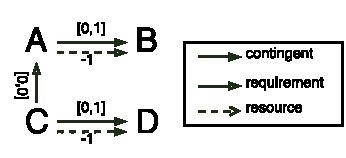
\includegraphics[width=0.43\textwidth,trim={0.23cm 0.23cm 0.00cm 0.37cm},clip]{stnu_counter}
\caption{TRN cannot select $\sigma$ dynamically. Number over a resource constraint arrow represents $r$ in a simple resource constraint.}
\label{fig:stnu_counter}
\end{center}
\end{figure}

Figure \ref{fig:stnu_counter} shows an example where $TRN$ would report no solution found. However, if we ignore the resource constraints and find a dynamic execution strategy satisfying temporal constraints, it never violate resource constraints, as they are both generating. The reason TRN fails to find the solution is due to the fact that $B$ and $D$ are both in the set $RE$ and TRN's solution attempts to fix the ordering between $B$ and $D$, which is impossible to do statically in this example.


% INPUT: atn N, {src} S (spanning N.timepoints)
% OUTPUT: scheduling strategy on N or fail
% ALGORITHM:
% X = subset of N.timepoints used by SRCs from S
% for every permutation pi of X:
% stcs = pi encoded by STCs
% result = N.solve_with_stcs(stcs)
% if result is schedule:
%        return schedule
%       fail
